\chapter{Intro}\label{ch:intro}

The boundary between Natural Language Processing (NLP), Text Generation (TG) and \textit{Neural Text Generation (NTP)}, is relatively blurred and overlap in many ways. Generally speaking, all of the NTG tasks are NLP based, but not all NLP tasks are NTG based.
NTG is the latest improvement of TG, because it applies the latest Deep Learning (DL) research achievements.

\section{Difference of NLP and NTG}
In recent months and years, neural networks have produced many \textit{state-of-the-art} results in almost all possible disciplines of machine learning \cite{NTG2}. The roots of Neural Networks (NN) lie down almost 80 years ago in 1943 when \textbf{McCulloch-Pitts} \cite{NN} compared for the first time neuronal networks with the structure of the human brain. This first attempt to approach artificial neurons with neurons from the brain leads to the nowadays commonly used understanding of a simple neuron of an underlying neural network (shown in figure \ref{neuron}). The connected neurons create an artificial neural network, which can calculate any possible logical or arithmetical function. 

\begin{figure}
  \begin{center}
  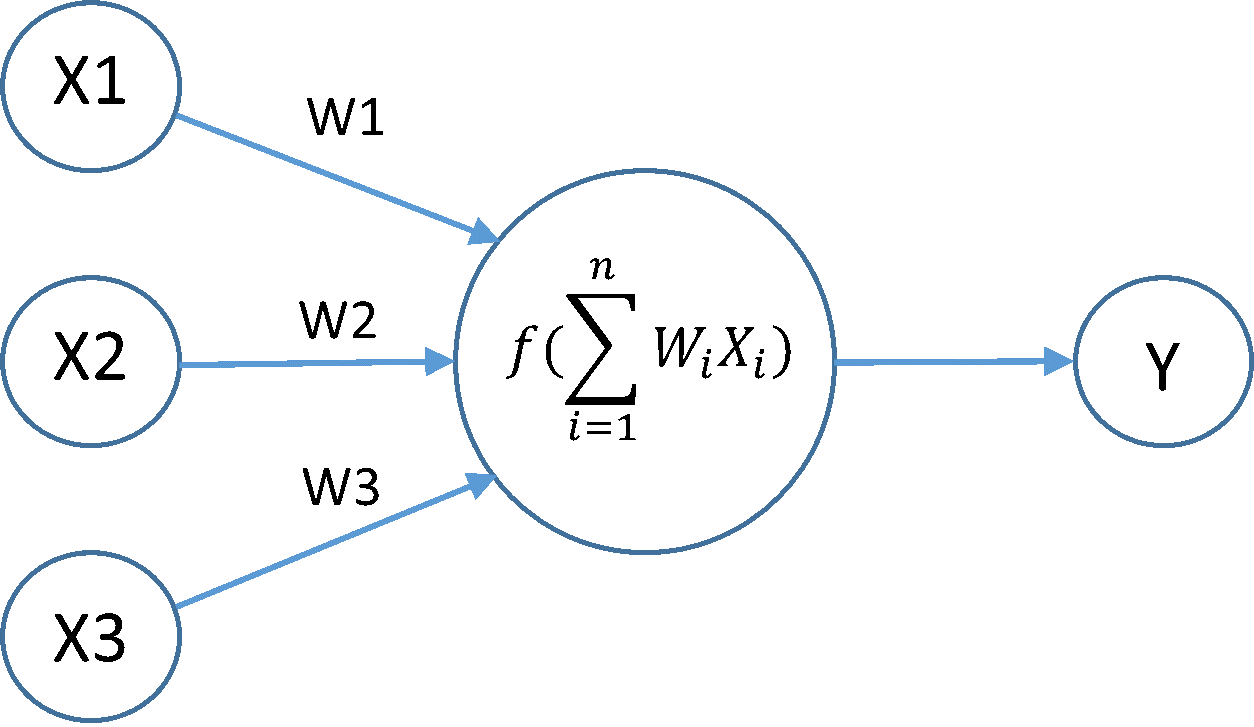
\includegraphics[width=3.5in]{photos/neuron}\\
  \caption{A simple Neuron with 3 inputs and 1 output \cite{neuron}}\label{neuron}
  \end{center}
\end{figure}

The range in which NN's (in the year 2020) apply to modern technologies is wide. Some disciplines have only been created due to the invention of neural networks because they solve existing- and new problems very effectively and efficiently. Many frequently held conferences around the globe contribute continuous evidence of the successes of neural networks. Among those various disciplines counts for example \textit{Pattern recognition} with Convolutional Neural Networks (CNN) \cite{cnn} or the famous \textit{CIFAR-10} dataset \cite{cifar}, where many amateurs \cite{tim} and experts attempt annually to further increase the accuracy of predicting the 10 different image classes. \\
The basis of this thesis's topic \textit{textgeneration} is Natural Language Processing, \textit{NLP} for short. This field covers many other hot research topics, such as 


\begin{itemize}
\item Sentiment Analysis
\item Machine Translation
\item Speech Recognition
\item Text Generation (Neural Text Generation \textit{NTG})
\item Chatbots
\end{itemize}

Another term for text generation is  \textit{Language Modelling}, because text generators use the words of a language and grammar as input for the model. In the past five years, primarly two approaches were used for modelling NLP, namely the \textbf{rule-based} system and the \textbf{template-based} system (Figure \ref{rules_based}) \cite{NTG2}. Today neural end-to-end systems are \textit{state-of-the-art} \cite{End_to_End}. These systems offer more flexibility and scale with proportionately better results, and less data is required because of the increased complexity. A major disadvantage is that the necessary computing power has increased exponentially. However, this leads to a complex problem because it becomes more and more challenging to understand the decisions of the neural network. The neural network is still, to a large extent, a \textit{black box}. Especially in NLP it gives surprisingly good results. The neural network models for text processing are difficult to understand, so nowadays, compromises between rule-based systems still have to be made, and hybrid systems are most commonly in use. 


\begin{figure}
  \begin{center}
  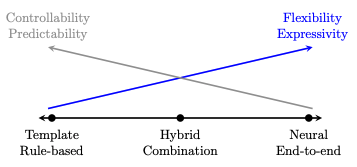
\includegraphics[width=3.5in]{photos/rule_based}\\
  \caption{Rule-Based vs. Neural-Text-Generations System \cite{NTG2}}\label{rules_based}
  \end{center}
\end{figure}

The neural text generation, also called \textit{NTG}, has many other exciting application fields, which overlap partly with NLP, including
\begin{itemize}
\item Speech recording and conversion to text
\item Conversation systems e.g. chatbots
\item Text summary
\item Caption generation
\end{itemize} 

In order to train language models properly, Deep Learning algorithms teach the model the probabilities of occurring words with respect to the preceding words. There are several approaches to achieve this goal. Language models can be trained on the level of words, whole sentences, or even whole paragraphs. The granularity in which the training takes place is called \textit{n-grams}, where \textit{n} represents the number of preceding words. Further explanation in subsection \ref{ss:ngram} of chapter \ref{ch:sota}.

\section{Case study of a current NLP system}

The following case introduces the underlying architecture of the famous \textbf{"Hey Siri"} command from Apple's \textit{Siri}. There are many fascinating use cases, but the most crucial hot research topics of 2019-2020 are introduced in chapter \ref{ss:trends}. Siri is a prime example because it combines two of the most relevant NLP tasks, namely Speech Recognition and Text Generation. Apple released the first version of Siri in 2011 with the iPhone 4s for the public costumers. At this time, users were still forced to press the \textit{Home Button} to give Siri a command via voice. For Siri to fulfill the user commands, it first needs to understand the human language itself by recognizing and splitting the words accordingly. Secondly, it needs to process those words further to a context and figure out what the user wants. 

\subsection{Hands-Free Access to Siri}
For the release of the iPhone 6 (iOS 8) in 2015, Apple upgraded Siri to a large extent. Without the need to interact with the iPhone physically, it can now detect the primary-users voice \textit{"Hey Siri"} to wake up automatically. Even though it might not sound like an innovation, still a lot is going on behind the scenes to create a flowless experience \cite{siri1}. 

The following figure \ref{flow} shows the entire process of detecting the wake-up sentence \textit{"Hey Siri"}.

\begin{figure}
  \begin{center}
  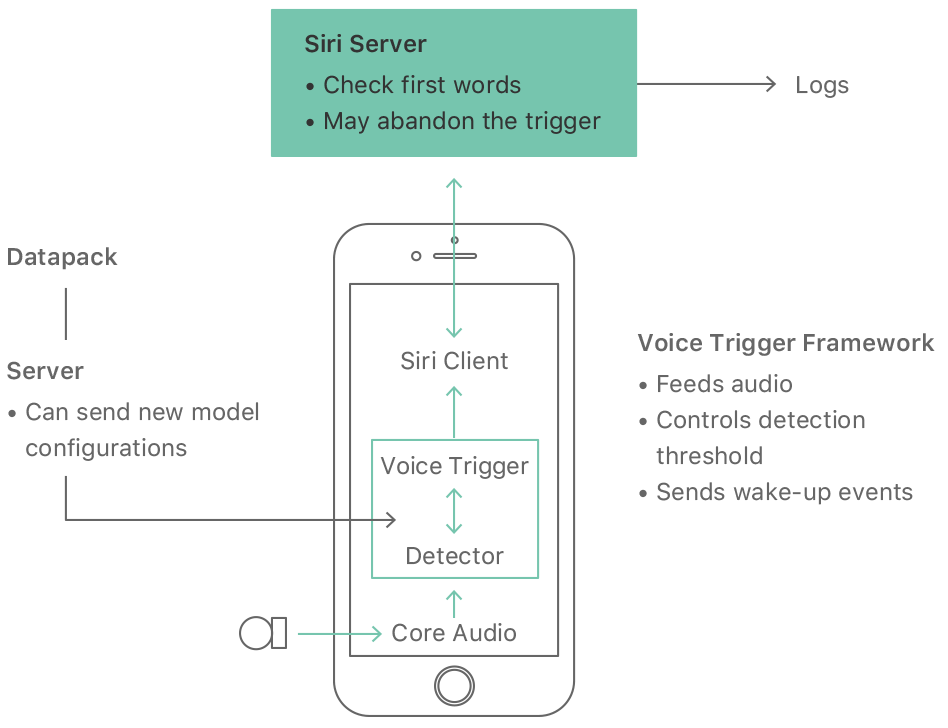
\includegraphics[width=4.5in]{photos/HeySiriFlow-1}\\
  \caption{The Hey Siri flow on iPhone (Apple 2017) \cite{siri1}}\label{flow}
  \end{center}
\end{figure}

For computing the error, there exist two different metrics. The false-accept rate (FAR) denotes the number of false activations which occur every hour, and the false-reject-rate (FRR) counts who often Siri is not activated when it was asked. Those objectives are essential to denote because machine learning and text generation tasks usually have loss function. The training aims to reduce the loss, in the case of Siri, Deep Learning aims to reduce the two different error rates. 
Deep Learning was applied with a network consisting of five hidden-layers. 

\begin{figure}
  \begin{center}
  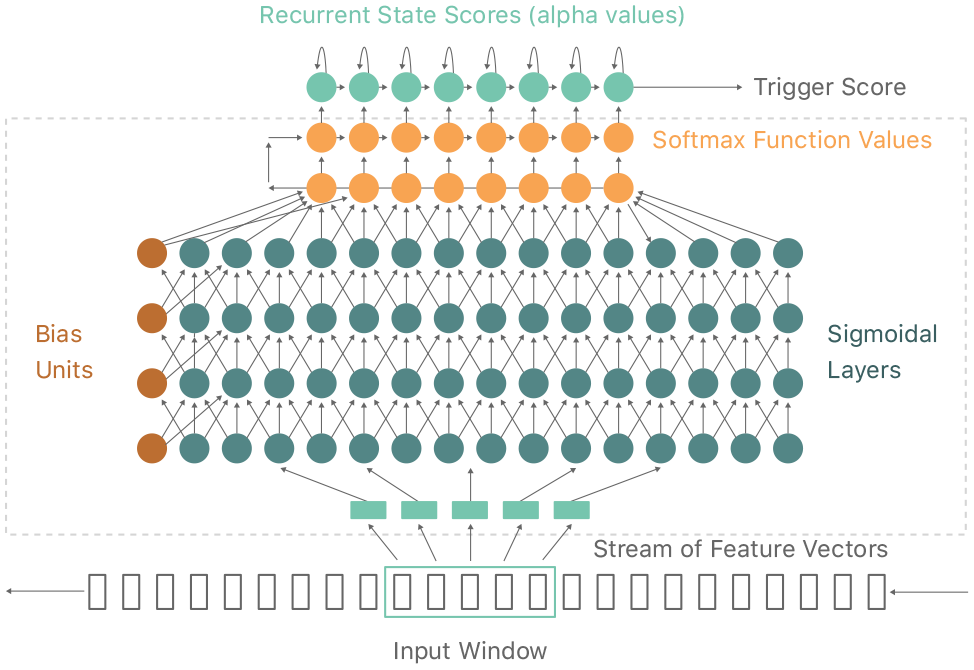
\includegraphics[width=4.5in]{photos/TrainingDNN-1}\\
  \caption{Structure of the DNN with Recurrent State Scores (Apple 2017) \cite{siri1}}\label{dnn}
  \end{center}
\end{figure}

The recurrent state scores (figure \ref{dnn}) are achieved through the use of Recurrent Neural Networks (RNN) \cite{siri2}, multi-style training, and curriculum learning. 
Recurrent Neural Networks (RNN) will be further explained in subsection \ref{ss:nn} of chapter \ref{ch:proto}. The spoken words are split into \textit{phonemes} consisting of all sounds in the corresponding spoken language. The network was trained on tons of data, according to Apple \cite{siri1}. With this training, this \textit{acustic model} is now able to funnel the user's voice through this network and distinguish whether the sentence was \textit{"Hey Siri"} or not. The core In figure \ref{flow} is this acoustic model. The iPhone microphone always listens and converts all sounds into a stream of waveform samples. Those samples are transformed into a sequence of frames, which describe approximately 0.01 seconds in time. Those frames are fed into the Deep Neural Network (DNN) acoustic model and produce a log probability to calculate the probability of the current sound being the \textit{"Hey Siri"} activation sentence. The network contains two different models, to further reduce the error rate by double-checking if the spoken sentence is understood properly. 
\\
Many companies tend to store their high-tech technologies like speech recognition and NLP applications recently on the cloud. Apple uses cloud technologies as well as \cite{siri1} for Siri because the team behind Siri faced limitations regarding the battery life and the computing capacity of the CPU of the iPhone. So, the wake-up neural network is stored locally on the iPhone, whereas the model for understanding the generating the output to a question is stored on the cloud.

\subsection{Personalized Hey Siri}
Siri can recognize the words \textit{"Hey Siri"}, but it responds to anyone, not only the primary user. To troubleshoot this error, Apple introduced the speaker recognition (SR) system.

The wake-up task is rather simple compared to figuring out the context, but still highly researched. When it comes to programming a model, the input language for this model gets split up into basically three parts as the first step\cite{siri2}.

\begin{itemize}
\item \textit{Syntax}: Composition of the phrases
\item \textit{Semantics}: Meaning of the phrases
\item \textit{Pragmatics}: Composition and context of the phrases
\end{itemize}

Siri gets activated when it recognizes the words \textit{"Hey Siri"}. The difference with the personalized system is that acoustic input now is further split up in the second step into the phonetic content, background recording environment, and the speaker's identity (personalization), as in figure \ref{siri1} (upper boxes) \cite{siri2}.

Siri is able to avoid unintended activations that sound similar but have a different meaning. Unintended activations are especially challenging, because people all over the world have different accents and dialects, depending on their origins. 

When the phone is configurated, in the \textit{enrolment stage}, the user is asked to repeat common phrases for a couple of times. This input is fed into a \textit{statistical model} for recognizing the user's voice. In the \textit{recognition stage}, the computer evaluates if the speech input fits the primary-users-trained model and accepts or rejects the request based on that decision.

	
\begin{figure}
  \begin{center}
  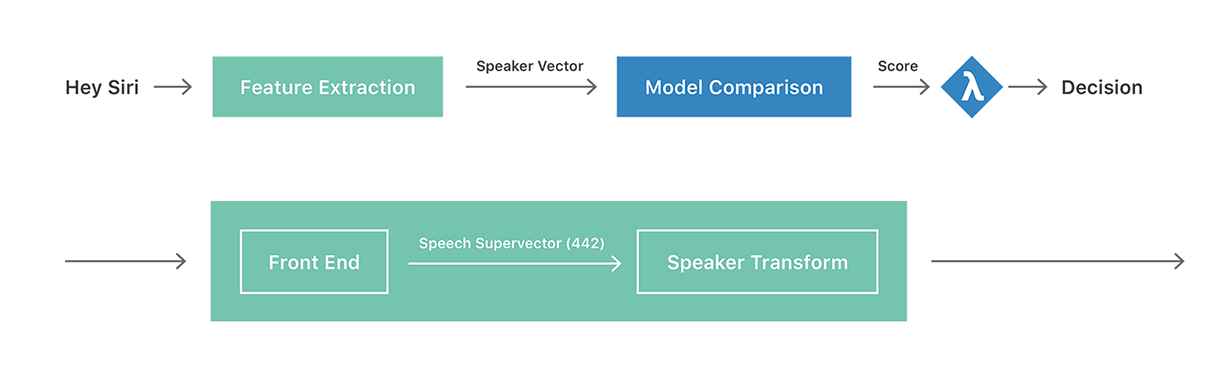
\includegraphics[width=4.5in]{photos/siri1}\\
  \caption{Block diagram of Personalized "Hey Siri" (Apple 2018)\cite{siri2}}\label{siri1}
  \end{center}
\end{figure}

Figure \ref{siri1} from Apple shows the fundamental diagram for this process \cite{siri2}. The \textit{Feature Extraction} computes a fixed-length speaker vector for the input sentence \textit{"Hey Siri"}. This vector contains information about phonetics, background noise, and the identity of the user. In the second step, the vector is transformed in such a way that the environmental background noise is reduced to a minimum with the help of the \textit{Fourier Transform}, and the user's identity is extracted.

In the early days, Apple used different algorithms to train the speech recognition models. Apple used for example the \textit{Linear Discriminant Analysis} (LDA) which scored very poor compared to the latest approach \textit{Deep Neural Networks} (DNN) \cite{siri1}. The research paper from Apple states that the DNN achieves a speaker recognition error rate of 4.3\%, whereas the LDA produces an 8.0\% error rate. This performance test was conducted with an overall performance test. This shows that the personalized models score with much higher accuracy than before.

\subsection{Regionally Specific Language Models for Speech Recognition}

Geo-Language-Models

\begin{figure}
  \begin{center}
  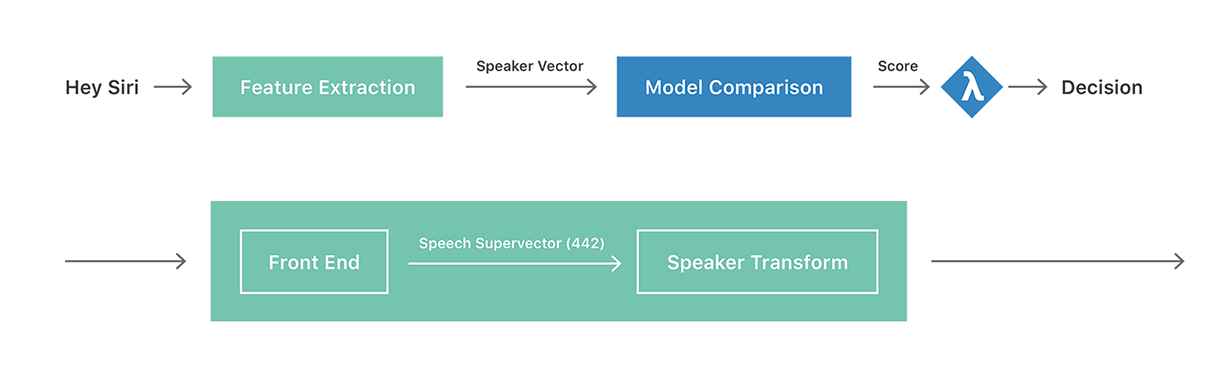
\includegraphics[width=4.5in]{photos/siri1}\\
  \caption{System Overview (Apple 2018)\cite{siri3}}\label{siri3}
  \end{center}
\end{figure}





